\documentclass[a4paper, 10pt]{article}
\usepackage[utf8]{inputenc} % Change according your file encoding
\usepackage{graphicx}
\usepackage{url}

%opening
\title{Seminar Report: Chatty}
\author{\textbf{Carles,Ricard}}
\date{\normalsize\today{}}

\begin{document}

\maketitle

\begin{center}
  \textbf{Carles Tornel}\\
  \textbf{Jesus Alfaro}\\
  \textbf{Ricard Abril}

\end{center}

\section{Introduction}

Aquesta pràctica tenia com a objectiu familiaritzar-se amb Erlang, programant la comunicació entre diferents nodes amb un servidor, o més, com intermediari. Vam haver de programar dos fitxers de servidors i un de client, que feiem servir per enviar missatges a altres clients.

\newpage
\section{Experiments}
\begin{enumerate}
  \item Make tests with different Sleep and Work parameters to  analyze  how  this  lock  implementation  responds  to  different  contention degrees.\\
  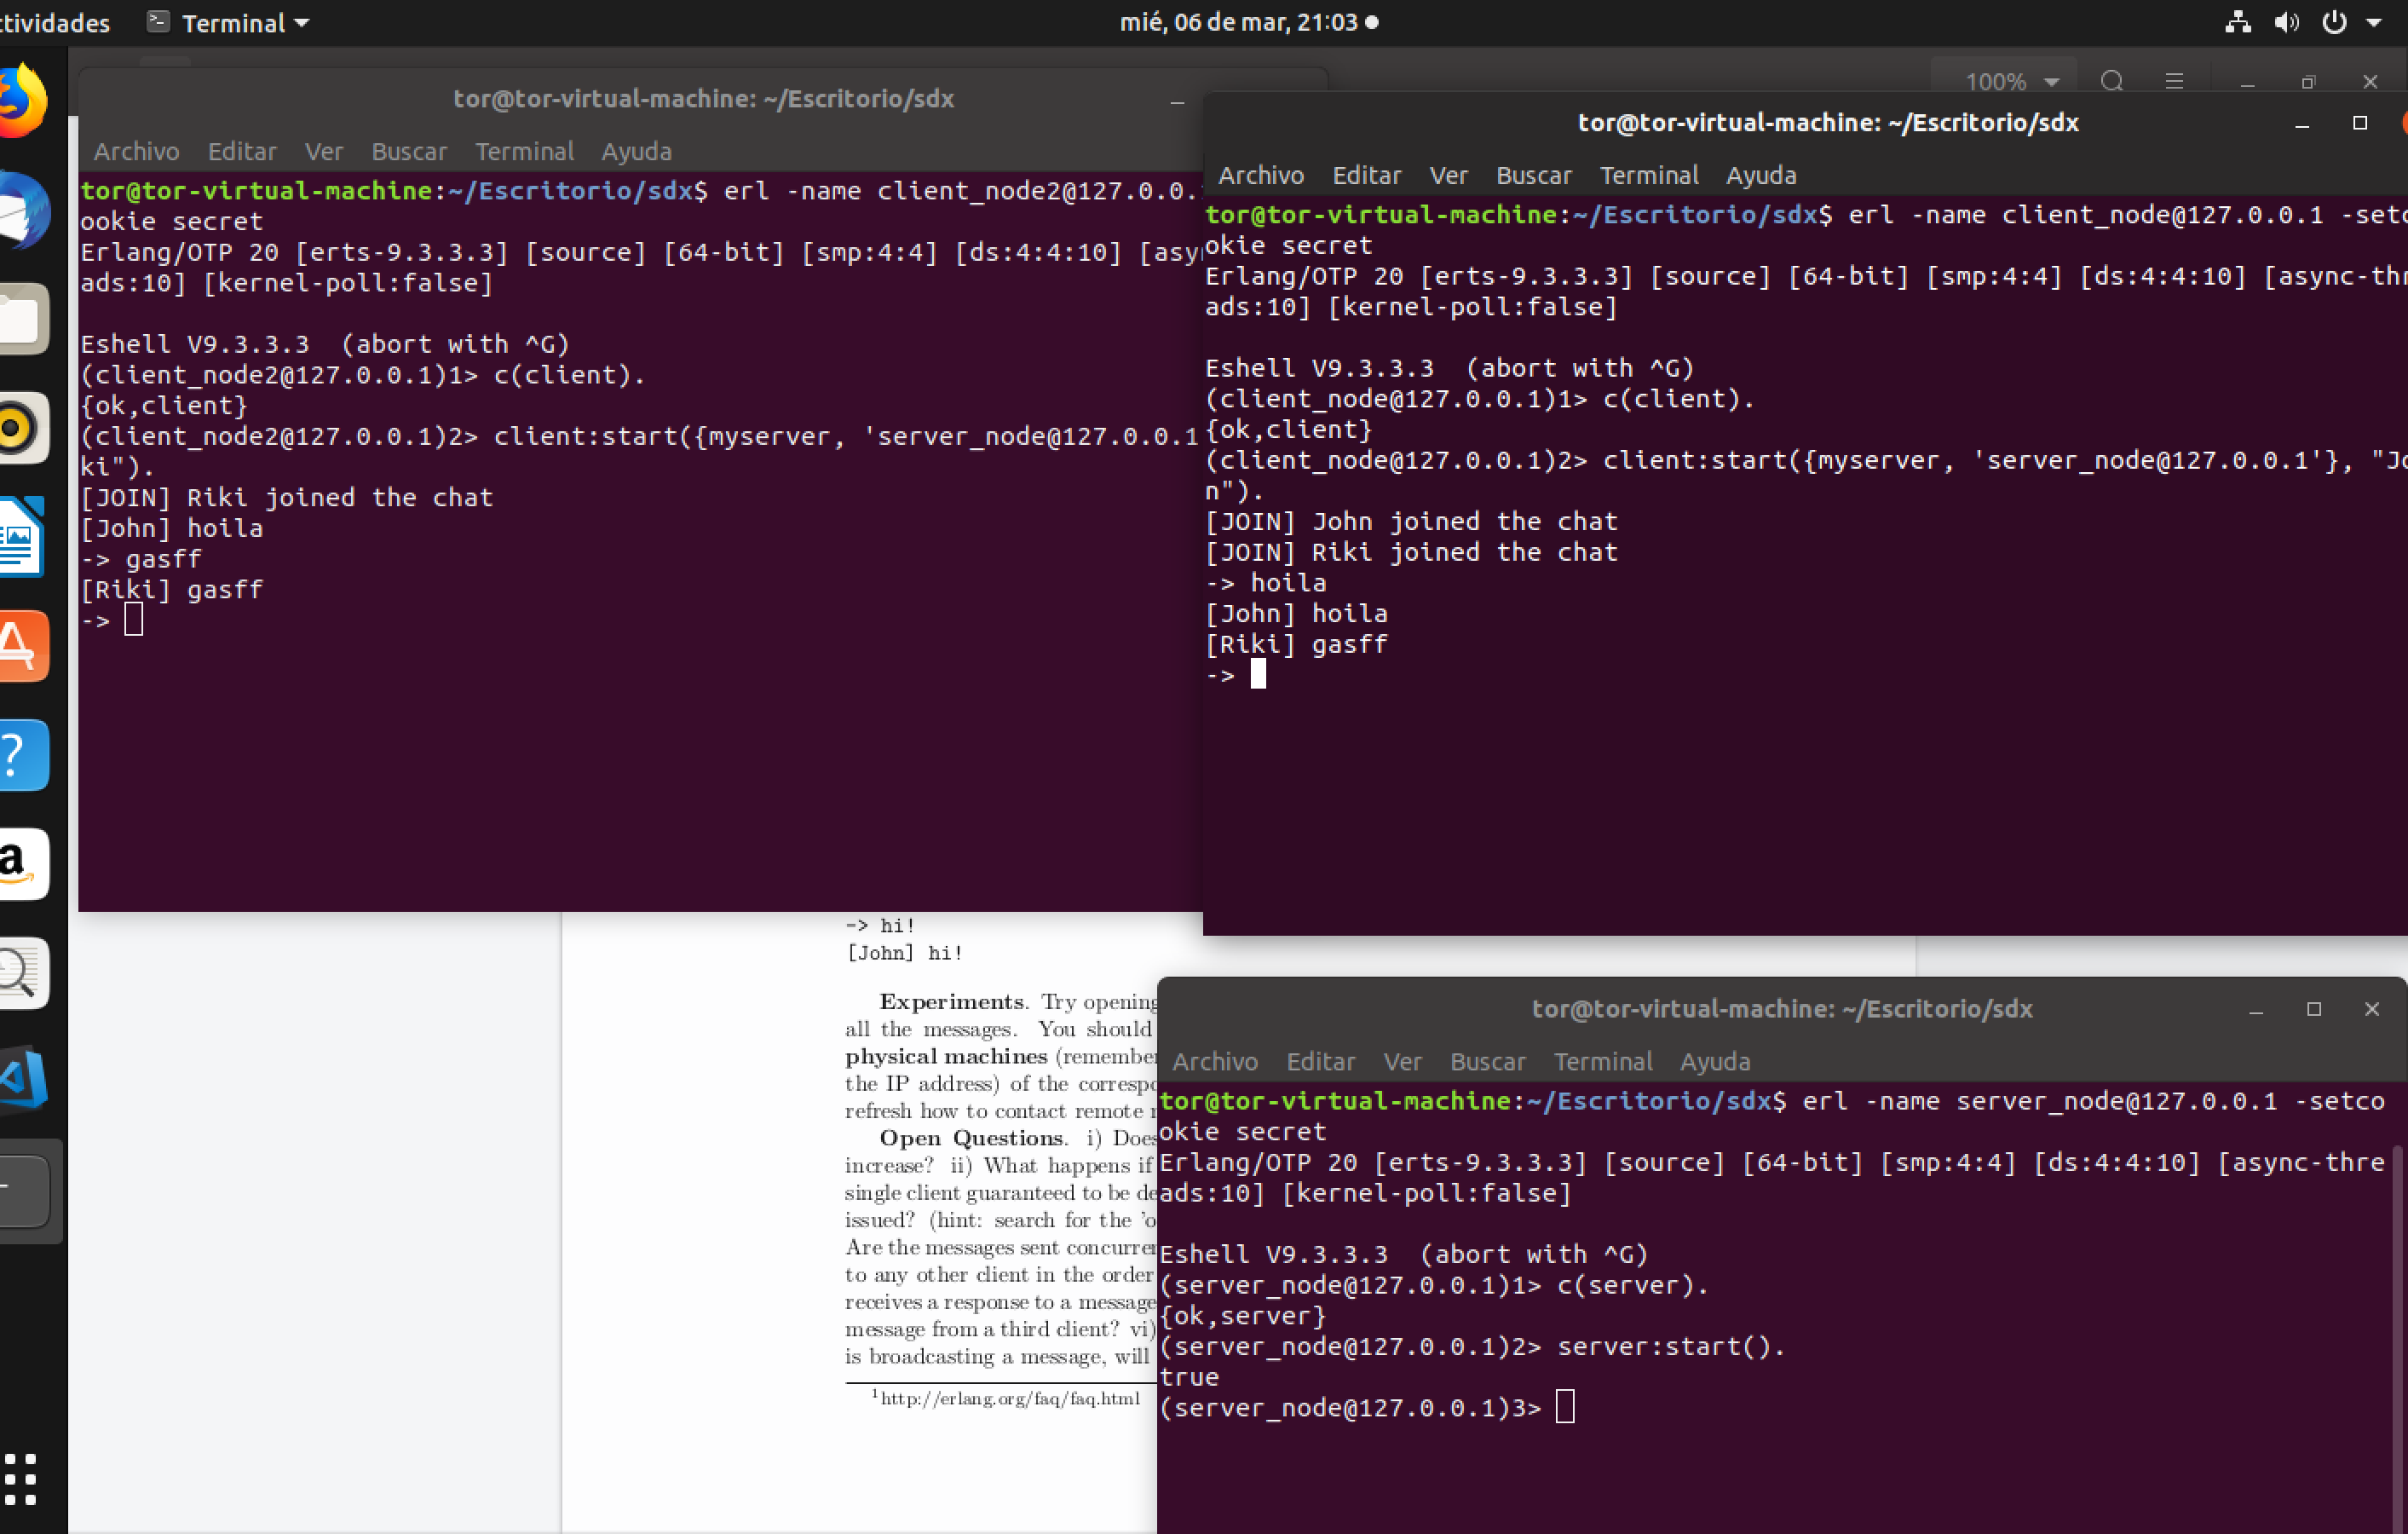
\includegraphics[width=\textwidth]{img1}\\\\


  \newpage\item Once you have a set of servers up and running, try connect- ing some clients to each of the server instances and begin to chat. Does it work? You can also try to crash some of the servers (e.g. by sending a disconnect message from the Erlang prompt) and see what happens.
  Al connectar diversos servidors i diversos usuaris a aquets, el chat segueix funcionant perfectament, de forma que encara estan en servidors diferents, tots els clients de tots els servidors podran veure els missatges de la resta. Tal i com es pot veure en la figura següent:\\\\\\
  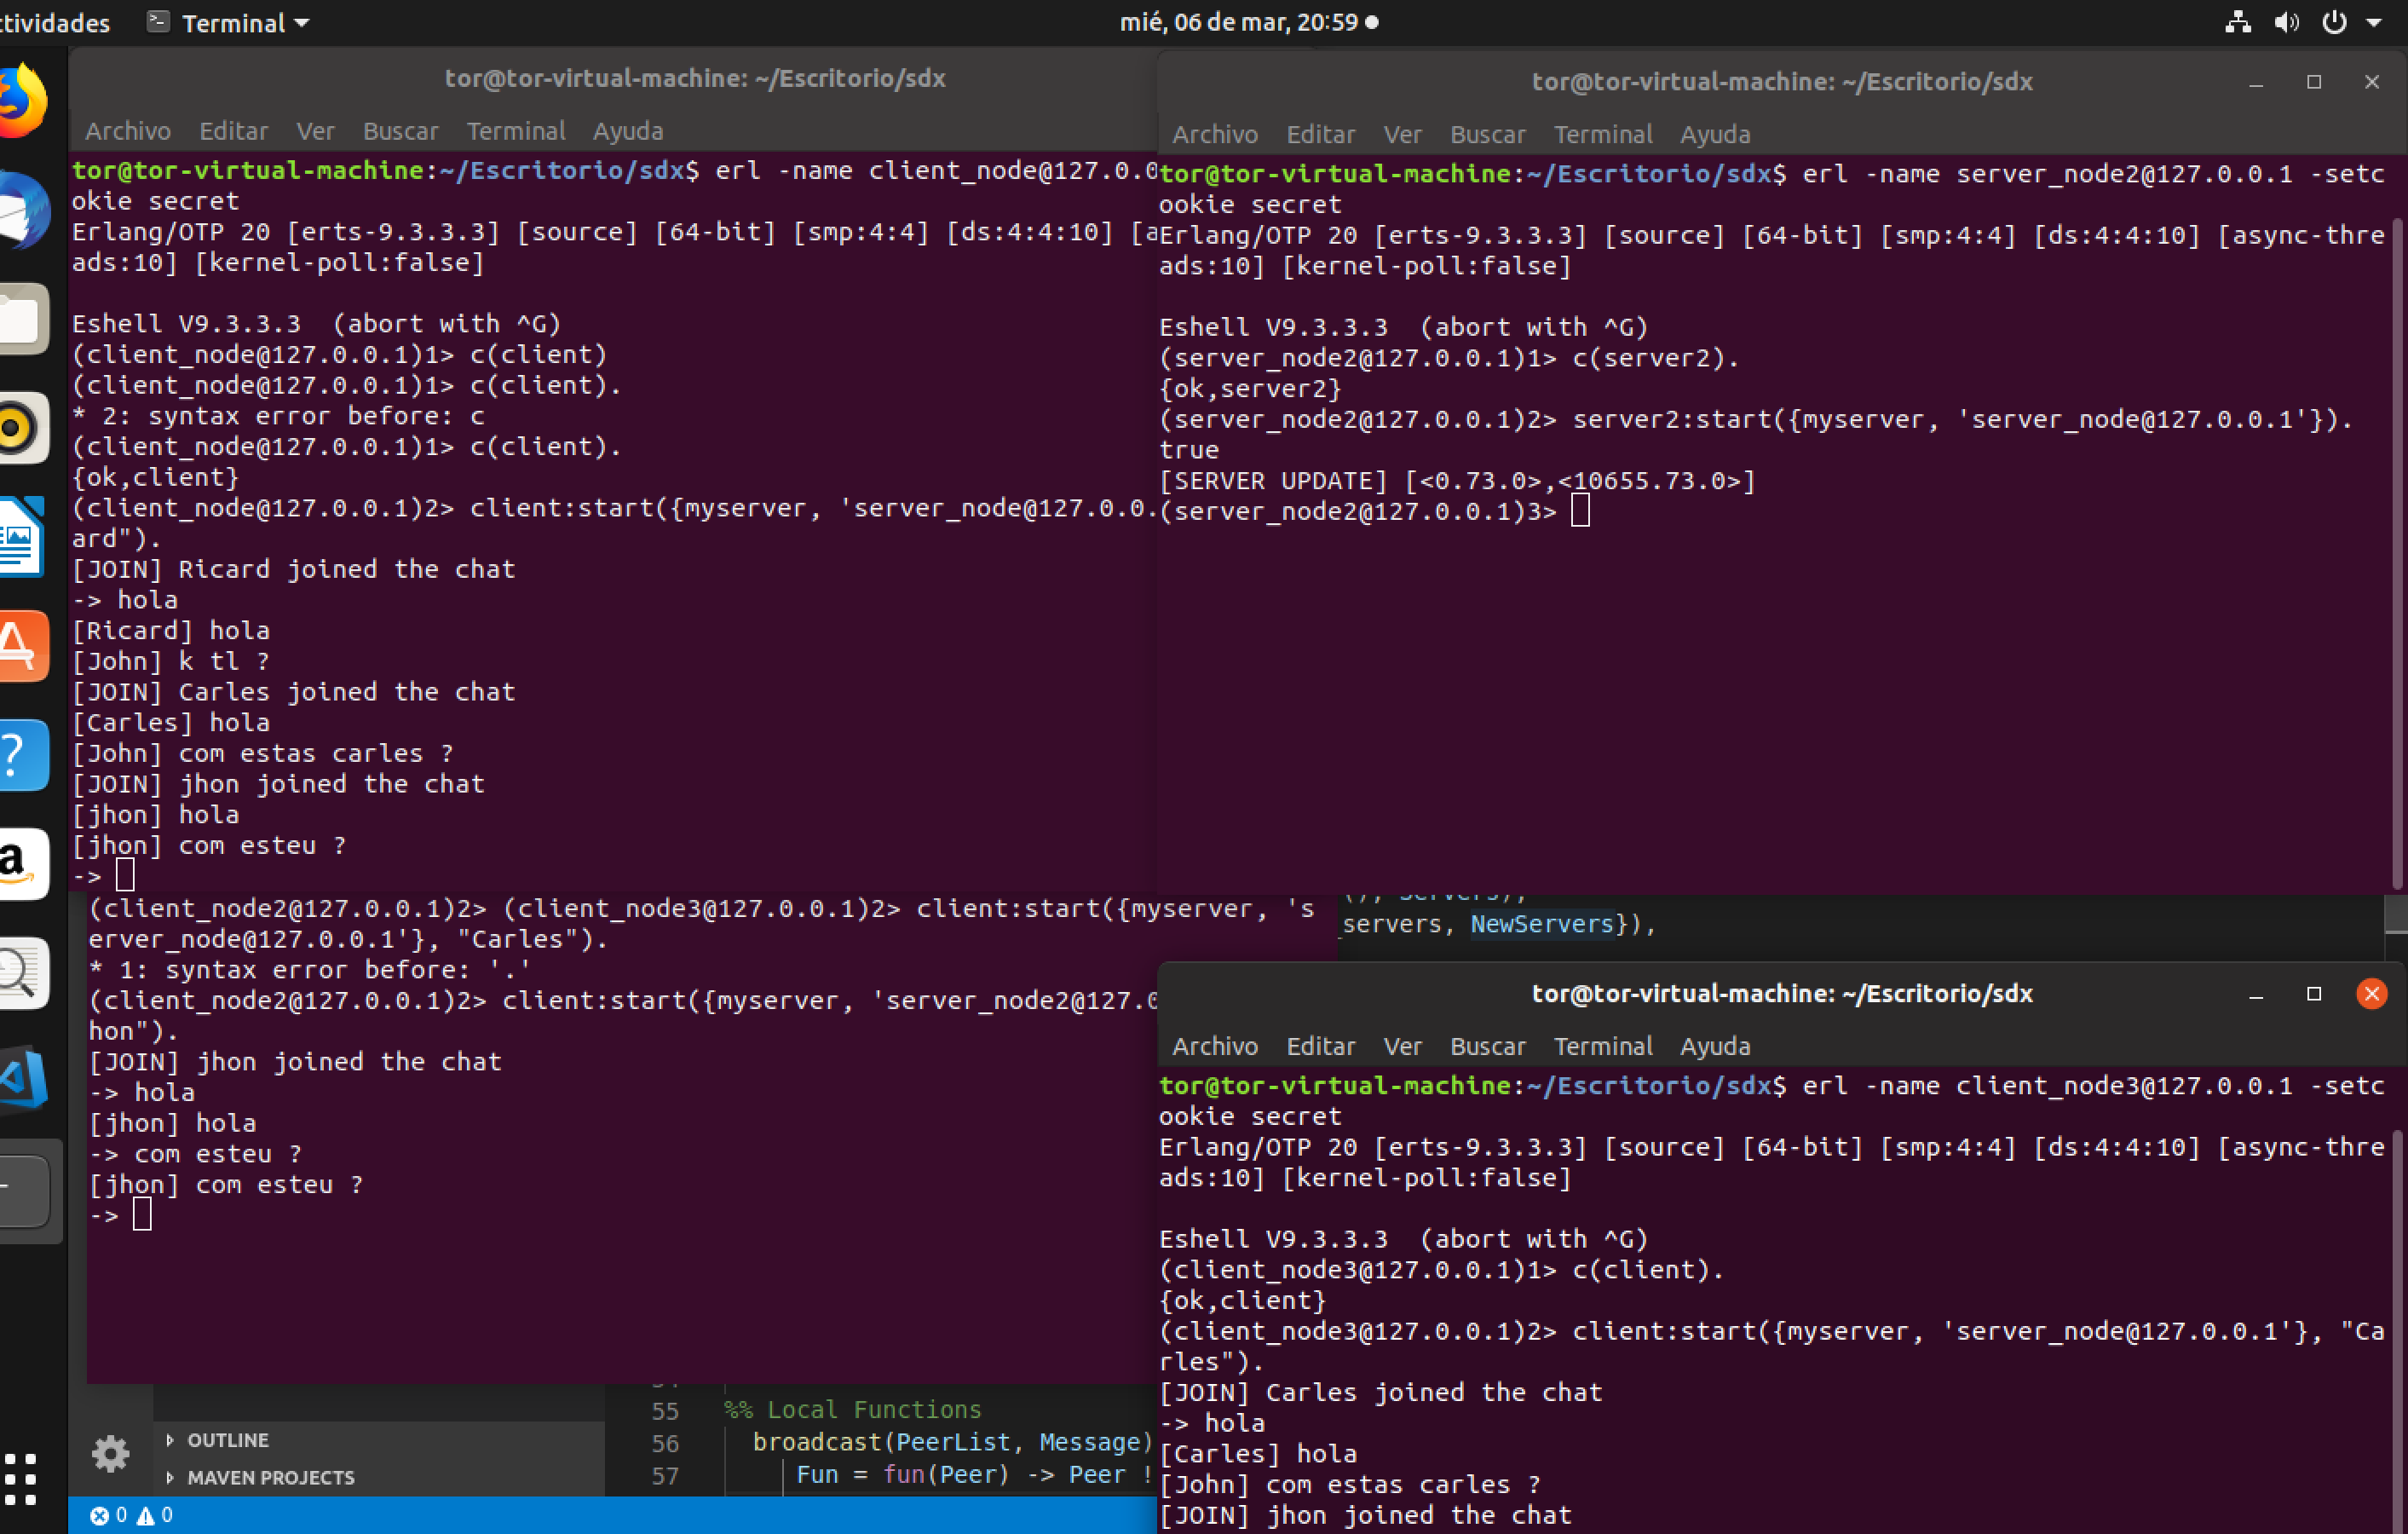
\includegraphics[width=\textwidth]{img2s}\\\\
 \newpage El tenir més d'un servidor, també aporta robustes al sistema, ja que si un dels servidors cau, nomes es queden sense connexió els clients que estan connectats en aquet servidor en específic. Tal i com es pot apreciar en les figures següents:\\\\
  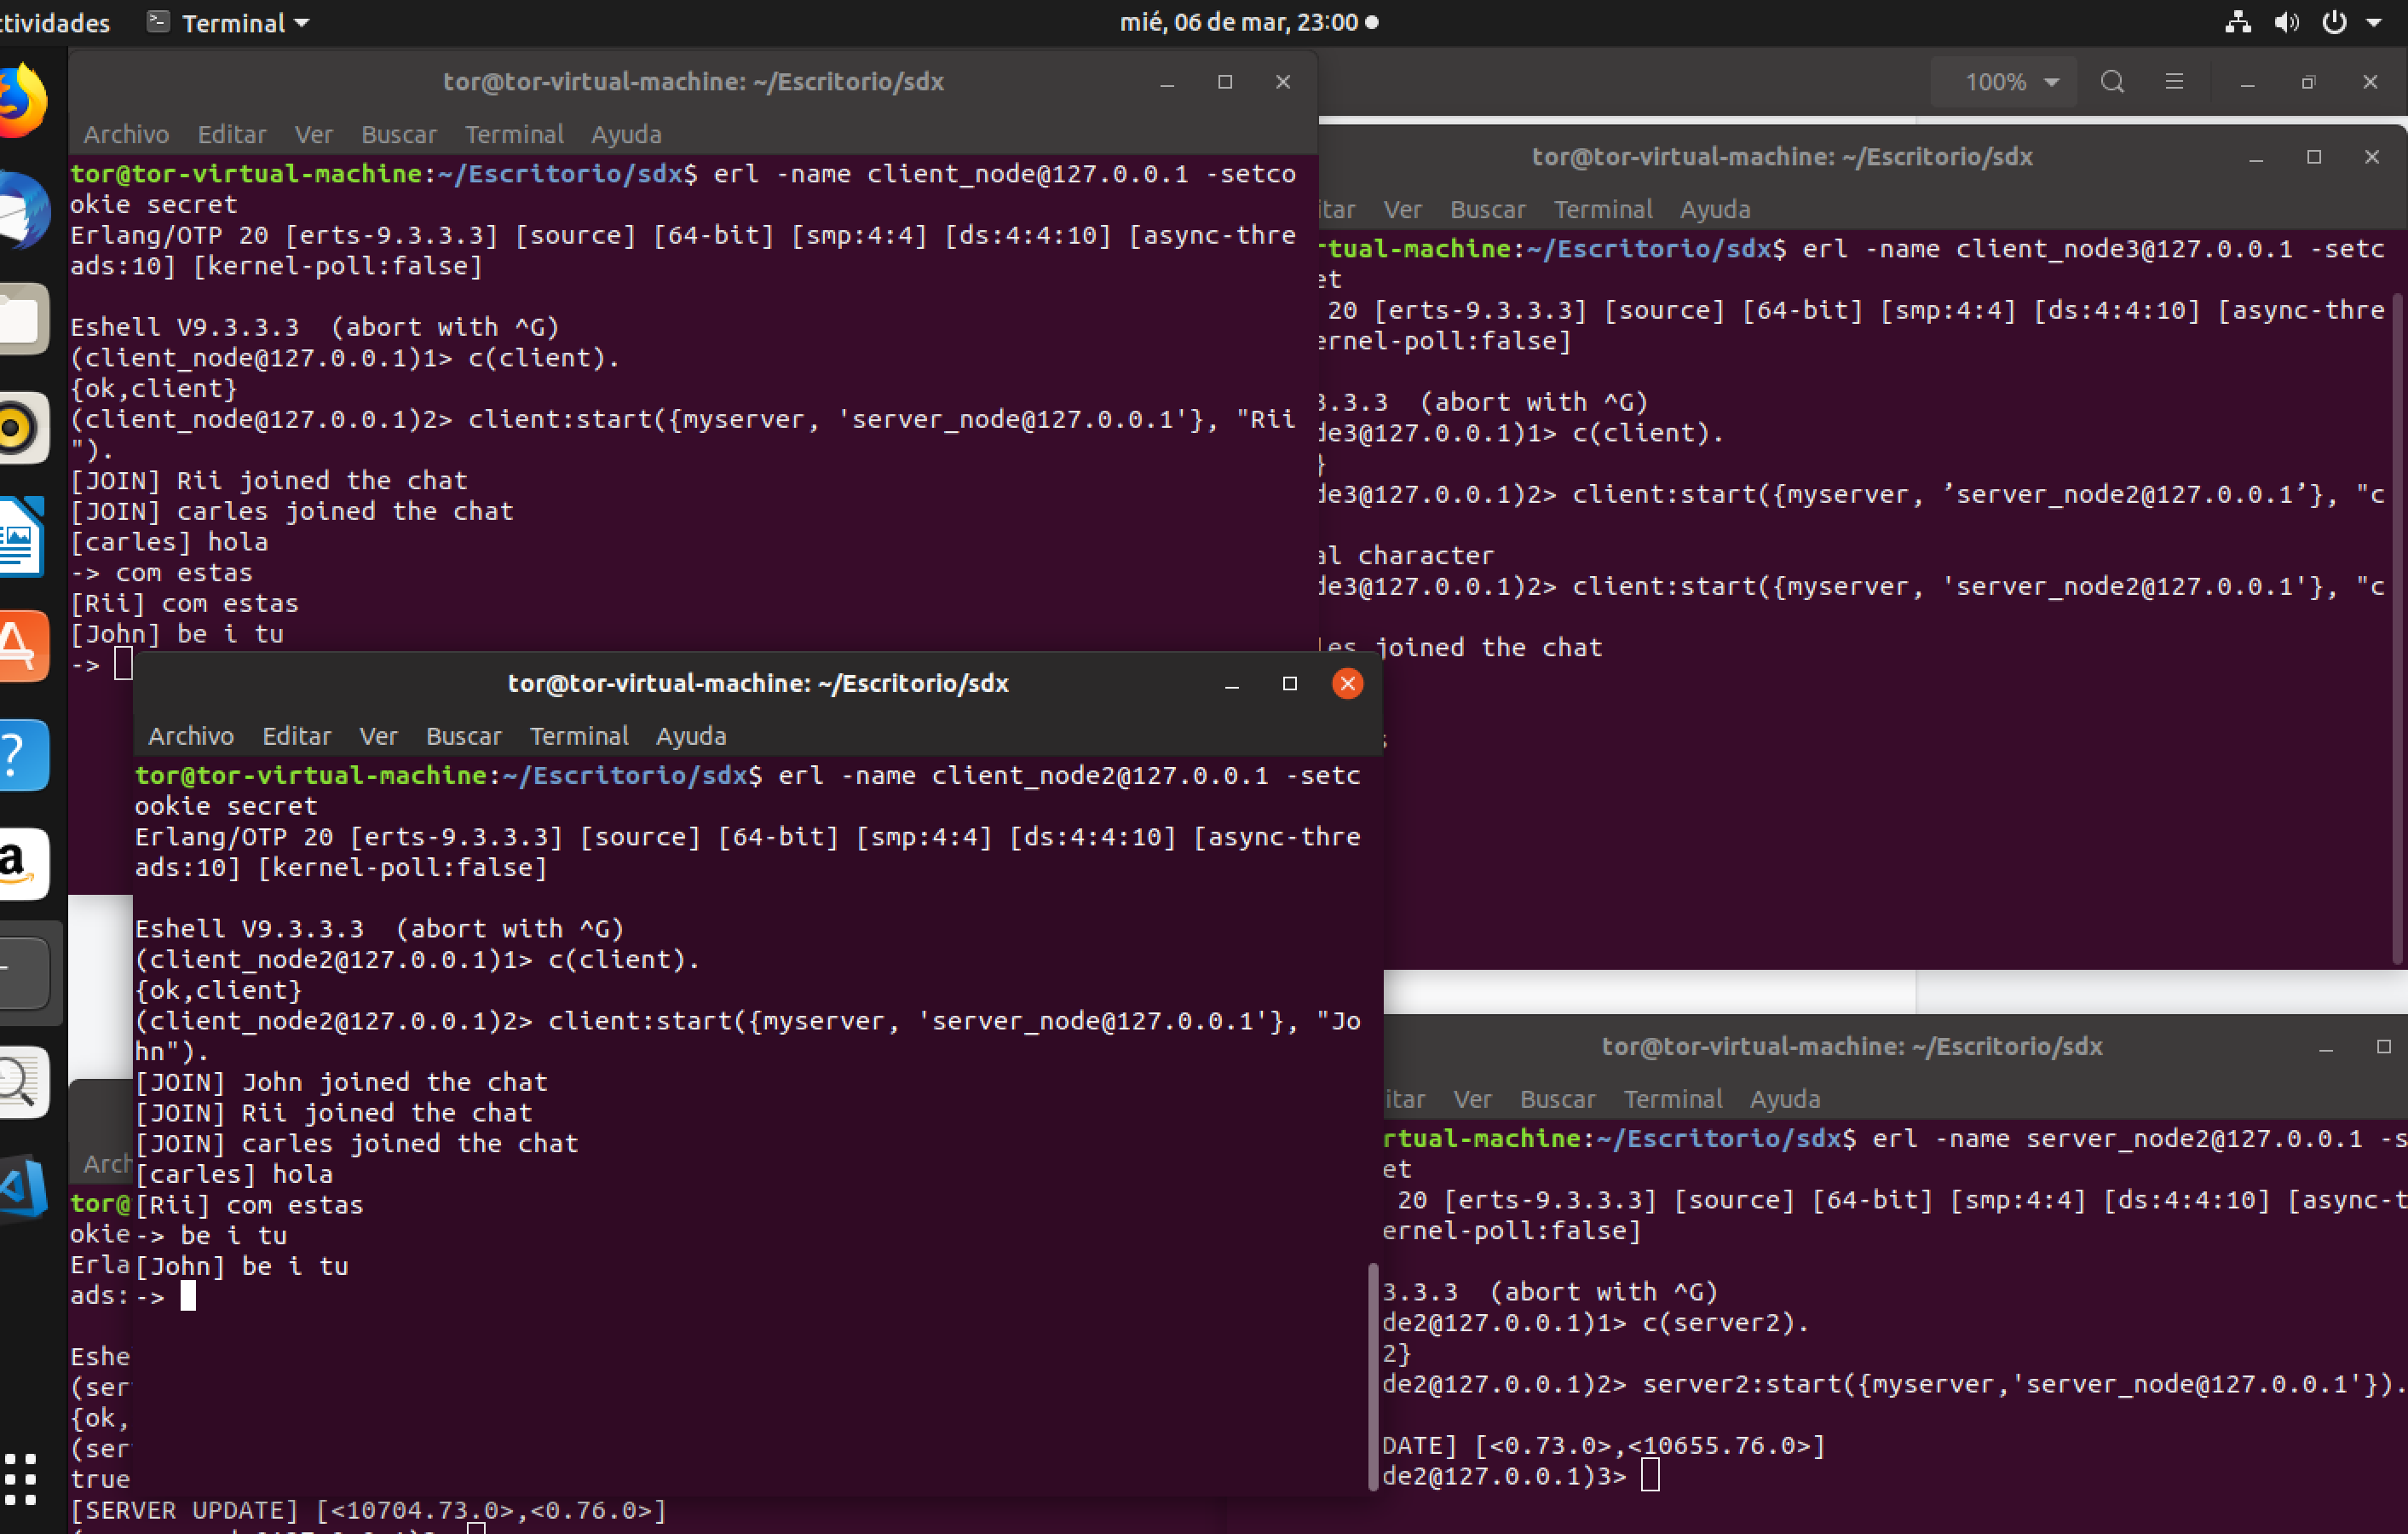
\includegraphics[width=\textwidth]{img3}\\\\
  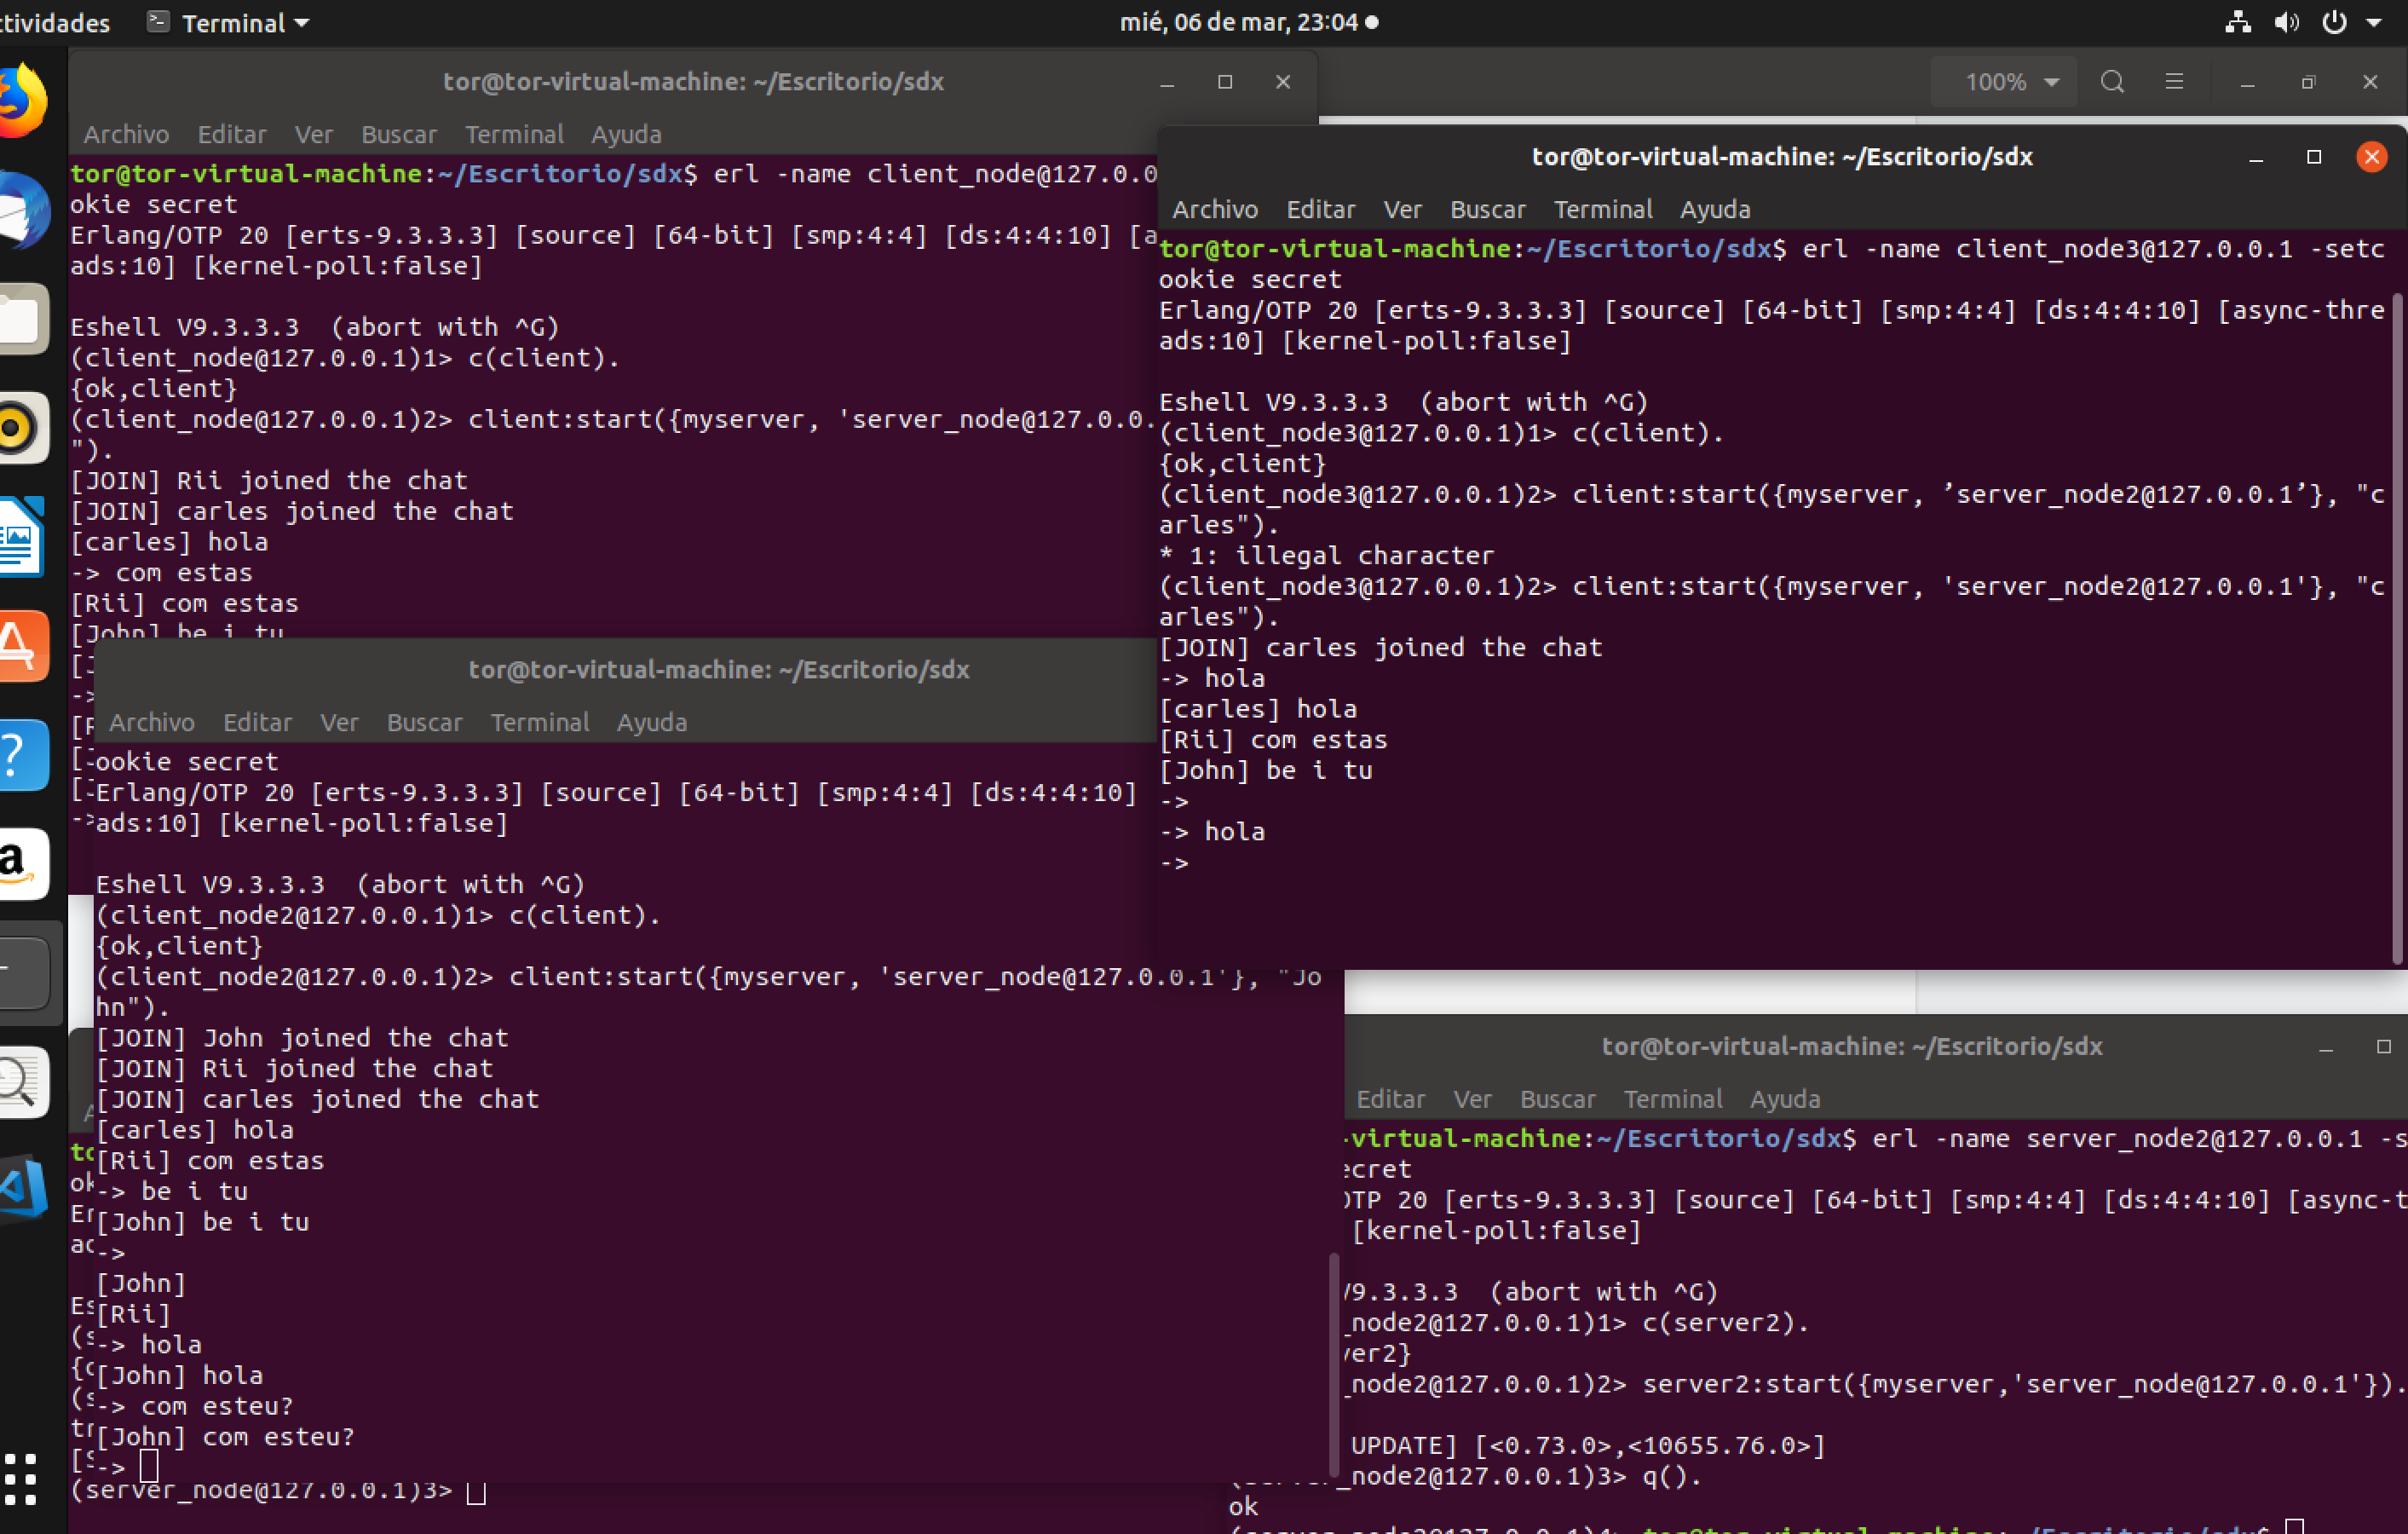
\includegraphics[width=\textwidth]{img4}\\\\
  
\end{enumerate}
\newpage
\section{Open questions}
\begin{enumerate}
\item
Does this solution scale when the number of users increase? \\
No, si el número d’usuaris incrementa. Un únic servidor no podrà mantenir el mateix rendiment i la qualitat del servei baixarà, ja que pot haver-hi saturació i coll d’ampolla.
 \item
 What happens if the server fails?\\
Aquest sistema només consta d'un únic servidor per gestionar els missatges, per tant, si el servidor falla, tot el sistema fallarà. No hi ha resiliència al sistema.

\item
Are the messages from a single client guaranteed to be delivered to any other client in the order they were issued? \\
 Sí perquè hi ha un únic servidor que reenviarà als clients els missatges en l’ordre que els rebi. 
 
\item Are the messages sent concurrently by several clients guaranteed to be delivered to any other client in the order they were issued?\\ 	 	 	
Erlang no garanteix l’ordre dels missatges, ja que això comportaria una sèrie de mecanismes i controls que el llenguatge no adopta.

\item Is it possible that a client receives a response to a message from another client before receiving the original message from a third client?\\
Com els clients estan connectats al mateix servidor, no seria possible aquest esdeveniment, ja que com que tampoc hi ha cap mena de retenció client-server, els missatges haurien d'arribar en el mateix ordre en què van ser enviats.

\item If a user joins or leaves the chat while the server is broadcasting a message, will he/she receive that message?\\
No, perquè el servidor per enviar missatges ha de registrar prèviament tots els clients que s'uneixen, i no ho pot fer a alhora que fa un broadcast.
\end{enumerate}
\newpage
\paragraph[bold]{Making it robust}
\begin{enumerate}
\item 
What happens if a server fails?\\
Els clients que estiguin connectats al servidor caigut es desconnectaran del xat. Per poder reincorporar-se hauran de connectar-se a l’altre servidor existent.

\item
Do your answers to previous questions iii, iv, and v still hold in this implementation?

Respecte les preguntes 3 i 4 de l’apartat anterior, no es pot assegurar en Erlang el correcte ordre dels missatges entre dos nodes si existeix més d’un procés. Respecte la pregunta 5, es pot donar el cas que descriu l’enunciat si la latència del missatge de resposta és inferior a la latència del missatge inicial. Per exemple: Un client A i un client B estan connectats a un servidor S1 i un client C (connectat a un servidor S2) envia un missatge inicial que serà respost per B. El client A (més proper a B que a C) veuria abans la resposta (feta per B) que el missatge inicial (fet per C) si la latència de C és superior que a la del seu company B.
\item
What might happen with the list of servers if there are concurrent requests from servers to join or leave the system?\\
La llista dels servidors s’aniria modificant al moment en que un servidor forma part del grup de servidors actius o al moment en que un servidor es desconnecta del grup. Això no suposaria cap inconvenient ja que la llista està capacitada per soportar variacions. Un únic problema que podria aparèixer seria la possible saturació de la xarxa de servidors i clients si les peticions fossen moltes i molt concurrents, però això ja depèn de les característiques d’aquesta. En cas d’aquest problema, s’ignorarien les peticions de unir-se i/o marxar i la llista continuaria com anteriorment. 
\newpage
\item
What are the advantages and disadvantages of this implementation regarding the previous one? (compare their scalability, fault tolerance, and message latency).\\
Aquest sistema presenta més escalabilitat que l’anterior ja que a l’existir diversos servidors, la càrrega de treball entre els diferents nodes es pot repartir i així s’evita que un servidor realitzi tota la càrrega del servei.
La tolerància a fallades incrementa considerablement, ja que no es depèn d’un sol servidor encarregat de la comunicació entre tots els clients, sinó que són diversos els encarregats a transmetre els missatges entre els nodes i si algun d’aquests falla, pot existir la possibilitat d’anar per un camí alternatiu o en el cas pitjor deixar desconnectats als clients d’aquell únic servidor.
La latència del missatge és variable i depèn de la proximitat física entre el servidor i un client. Dos clients connectats a un mateix servidor tindran una latència més baixa que si un client i un altre client a un altre servidor s’intercanvien missatges. Tot i així, l’existència de més d’un servidor per on poder transportar els missatges provoca un alliberament de tràfic de la xarxa que pot reduir la latència efectiva del sistema.


\end{enumerate}

\section{Personal opinion}
L’implementació d’un xat com a primera pràctica de l’assignatura fa que es pugui apreciar, de manera interactiva i amb exemples, com funcionen a petita escala les xarxes distribuïdes i els seus principals aspectes i avantatges de la seva utilització, així com el paper de client-servidor i tots els passos que segueixen per poder-se comunicar.

\end{document}
